\section{Modern Second-order methods and nonconvex optimization}

\subsection{Cubic Regularization}

Motivation: for $L$-Lipschitz Hessian as in the assumption of Newton's method, we have $f(x) \le f(x_t) + \nabla f(x_t)^\top (x-x_t) + \frac{1}{2}(x-x_t)^\top \nabla^2 f(x_t) (x- x_t) + \frac{L}{6}\|x-x_t\|^3$. Similar to GD which minimizes the upper bound given by smoothness (Lipschitz gradient), cubic regularization is to minimize the upper bound given by Lipschitz Hessian. Algorithm: $x_{t+1} = \argmin_x f(x_t) + \nabla f(x_t)^\top (x-x_t) + \frac{1}{2}(x-x_t)^\top \nabla^2 f(x_t) (x- x_t) + \frac{L}{6}\|x-x_t\|^3$. This can be reduced to a convex problem.

\textbf{Convergence rate}: $\min_{i\le t} \|\nabla f(x_i)\| = O(t^{-2/3})$. If convex, we have $f(x_t) - f^* = O(t^{-2})$.

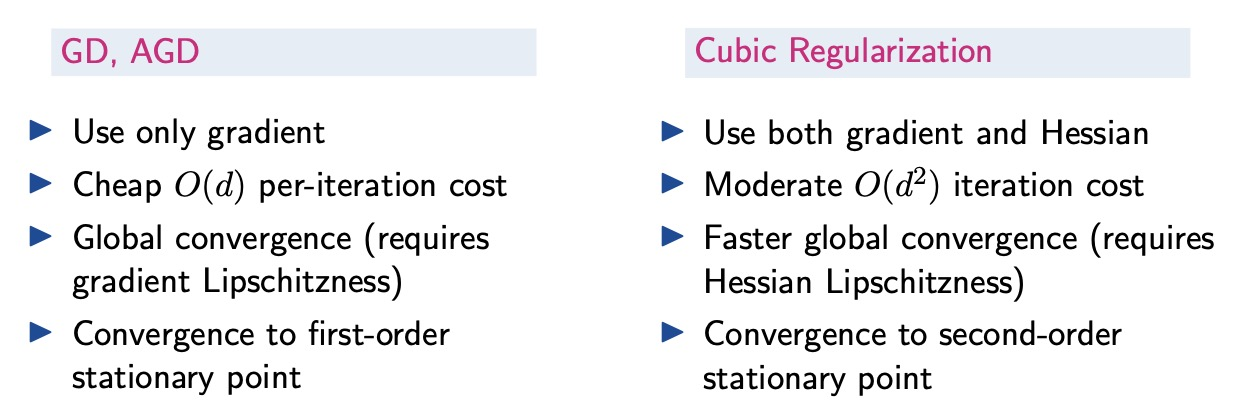
\includegraphics[width=\linewidth]{imgs/cubic.jpg}

\subsection{Nonconvex Optimization}

A nonconvex optimization may have exponentially many local minima, and determining whether a critical point is a local minimum is co-NP complete.

\textbf{Classification of stationary points}: (1) If $\nabla^2 F(x) \succ 0$, then $x$ is a local minimum; (2) If $\nabla^2 F(x) \prec 0$, then $x$ is a local maximum; (3) If $\nabla^2 F(x)$ has both positive and negative eigenvalues, then $x$ is a (strict) saddle point; (4) Otherwise, it remains inconclusive.

\textbf{Analysis}:
\begin{enumerate}
    \item \textbf{SGD converges to a stationary point}: see (12.8).
    \item \textbf{SGD with random initialization}: with random initialization, GD converges to a local minimum almost surely.
    \item \textbf{Noisy SGD}: with extra noise added to the SGD update, if $f$ satisfies strict saddle property and has Lipschitz Hessian, then noisy SGD converges to a second-order stationary point.
    \item \textbf{Benign landscapes}: if the function satisfies PL condition, or all local minimum is global minimum, then GD (in the latter case requires random initialization) converges to the global minimum.
\end{enumerate}